% version 1.00, date 12/11/16, auteur Kafui Atanley
Ce chapitre présente les maquettes pour chaque fonctionnalité pour chaque fonctionnalité additionnelle du lot 3 par rapport au lot 2.


\section{Fonctionnalité 8}
Ce paragraphe décrit les maquettes concernant la fonctionnalité 8 soit la géolocalisation. \\

La figure suivante \ref{maquette8-1} montre la maquette d'une fiche descriptive d'une entité possédant une adresse. Un espace devra être réservé pour afficher la location de l'entité comme visible sur la fmaquette.
\begin{figure}[H]
	\centering
	\includegraphics[scale=0.40]{images/maquettes/fonctionnalite9Geolocalisation.png}
	\caption{Maquette~: Fiche descriptive d'une entité possédant une adresse}
	\label{maquette8-1}
\end{figure}
La figure suivante \ref{maquette8-2} présente la maquette des filtres de tri attendus sur la géolocalisation dans les pages permettant de lister les entités.
\begin{figure}[H]
	\centering
	\includegraphics[scale=0.40]{images/maquettes/fonctionnalite9Filtre.png}
	\caption{Maquette~: Modèle de filtre attendues dans les liste de tri}
	\label{maquette8-2}
\end{figure}

\section{Fonctionnalité 9}
Ce paragraphe décrit les maquettes concernant la fonctionnalité 9 soit l'attribution de frimousse. \\

La figure suivante \ref{maquette9-1} montre l'email type de prise en charge d'une intervention de type frimousse.
\begin{figure}[H]
	\centering
	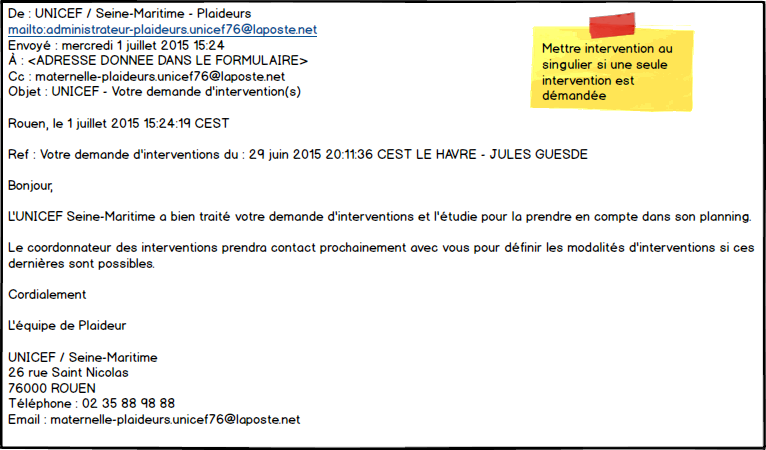
\includegraphics[scale=0.35]{images/maquettes/fonctionnalite5MailDePriseEnCharge.png}
	\caption{Maquette~: Email type de prise en charge}
	\label{maquette9-1}
\end{figure}
 L'utilisateur pourra s'attribuer une intervention de type frimousse via la liste d'intervention ou via la fiche descriptive de cette intervention.


\section{Fonctionnalité 10}
Ce paragraphe décrit les maquettes concernant la fonctionnalité 10 soit la gestion des ventes. \\

La figure suivante montre la maquette \ref{maquette10-5} de la page permettant d'ajouter une vente .
\begin{figure}[H]
	\centering
	\includegraphics[scale=0.40]{images/maquettes/fonctionnnalite10AjouterVente.png}
	\caption{Maquette~: Ajouter une vente}
	\label{maquette10-5}
\end{figure}

La figure suivante \ref{maquette10-3} montre la maquette de la page de la fiche descriptive d'une vente.
\begin{figure}[H]
	\centering
	\includegraphics[scale=0.40]{images/maquettes/fonctionnnalite10ConsulterVente.png}
	\caption{Maquette~: Consulter la fiche descriptive d'une vente}
	\label{maquette10-3}
\end{figure}

La figure suivante \ref{maquette10-4} Listing des ventes montre la maquette de la page permettant d'effectuer le listing des ventes.
\begin{figure}[H]
	\centering
	\includegraphics[scale=0.40]{images/maquettes/fonctionnalite10Ventes.png}
	\caption{Maquette~: Listing des ventes}
	\label{maquette10-4}
\end{figure}

La figure suivante \ref{maquette10-4} Listing des ventes montre la maquette de la page permettant d'effectuer le listing des ventes.

Il est possible de supprimer une vente à partir de la fiche descriptive d'une vente 


